\documentclass{report}
\usepackage[utf8]{inputenc} % Input UTF8
\usepackage[T1]{fontenc} % Fontes T1
\usepackage[overload]{textcase}
\usepackage[backend=biber, style=ieee]{biblatex} % para usar bibliografia
\addbibresource{bibliografia.bib}
\usepackage{csquotes}
\usepackage[portuguese]{babel} %Usar língua portuguesa
\usepackage{blindtext} % Gerar texto automaticamente
\usepackage[printonlyused]{acronym}
\usepackage{hyperref} % para autoref
\usepackage{graphicx}
\usepackage{color} 
\usepackage{listings} 
\usepackage{float}
\usepackage{setspace} 
\usepackage{indentfirst}
\usepackage{tcolorbox}
\usepackage[bottom]{footmisc} %passar a footnote para o fundo da página

\newenvironment{changemargin}[2]{%
\begin{list}{}{%
\setlength{\topsep}{0pt}%
\setlength{\leftmargin}{#1}%
\setlength{\rightmargin}{#2}%
\setlength{\listparindent}{\parindent}%
\setlength{\itemindent}{\parindent}%
\setlength{\parsep}{\parskip}%
}%
\item[]}{\end{list}}
%%
\usepackage{amsthm}

\theoremstyle{remark}
\newtheorem*{nota}{Nota}
%%%


\lstset{literate=
  {á}{{\'a}}1 {é}{{\'e}}1 {í}{{\'i}}1 {ó}{{\'o}}1 {ú}{{\'u}}1
  {Á}{{\'A}}1 {É}{{\'E}}1 {Í}{{\'I}}1 {Ó}{{\'O}}1 {Ú}{{\'U}}1
  {à}{{\`a}}1 {è}{{\`e}}1 {ì}{{\`i}}1 {ò}{{\`o}}1 {ù}{{\`u}}1
  {À}{{\`A}}1 {È}{{\'E}}1 {Ì}{{\`I}}1 {Ò}{{\`O}}1 {Ù}{{\`U}}1
  {ä}{{\"a}}1 {ë}{{\"e}}1 {ï}{{\"i}}1 {ö}{{\"o}}1 {ü}{{\"u}}1
  {Ä}{{\"A}}1 {Ë}{{\"E}}1 {Ï}{{\"I}}1 {Ö}{{\"O}}1 {Ü}{{\"U}}1
  {â}{{\^a}}1 {ê}{{\^e}}1 {î}{{\^i}}1 {ô}{{\^o}}1 {û}{{\^u}}1
  {Â}{{\^A}}1 {Ê}{{\^E}}1 {Î}{{\^I}}1 {Ô}{{\^O}}1 {Û}{{\^U}}1
  {ã}{{\~a}}1 {ẽ}{{\~e}}1 {ĩ}{{\~i}}1 {õ}{{\~o}}1 {ũ}{{\~u}}1
  {Ã}{{\~A}}1 {Ẽ}{{\~E}}1 {Ĩ}{{\~I}}1 {Õ}{{\~O}}1 {Ũ}{{\~U}}1
  {œ}{{\oe}}1 {Œ}{{\OE}}1 {æ}{{\ae}}1 {Æ}{{\AE}}1 {ß}{{\ss}}1
  {ű}{{\H{u}}}1 {Ű}{{\H{U}}}1 {ő}{{\H{o}}}1 {Ő}{{\H{O}}}1
  {ç}{{\c c}}1 {Ç}{{\c C}}1 {ø}{{\o}}1 {å}{{\r a}}1 {Å}{{\r A}}1
  {€}{{\euro}}1 {£}{{\pounds}}1 {«}{{\guillemotleft}}1
  {»}{{\guillemotright}}1 {ñ}{{\~n}}1 {Ñ}{{\~N}}1 {¿}{{?`}}1 {¡}{{!`}}1 
}
\begin{document}
%%
% Definições
%
\def\titulo{Guess the number - AP2}
\def\data{30-05-2021}
\def\autores{Diogo Matos, Miguel Gomes}
\def\autorescontactos{(102848) dftm@ua.pt, (103826) mig.gom@ua.pt}
\def\versao{1.0}
\def\departamento{DETI}
\def\empresa{Universidade de Aveiro}
\def\logotipo{ua.pdf}
%
%%%%%% CAPA %%%%%%
%
\renewcommand{\contentsname}{Índice}
\begin{titlepage}

\begin{center}
%
\vspace*{50mm}
%
{\Huge \titulo}\\ 

\vspace{10mm}
%
{\Large \empresa}\\
%
\vspace{10mm}
%
{\LARGE \autores}\\ 
%
\vspace{30mm}
%
\begin{figure}[h]
\center
\includegraphics{\logotipo}
\end{figure}
%
\vspace{30mm}
\end{center}
%
\begin{flushright}
\versao
\end{flushright}
\end{titlepage}

%%  Página de Título %%
\title{%
{\Huge\textbf{\titulo}}\\
{\Large \departamento\\ \empresa}
}
%
\author{%
    \autores \\
    \autorescontactos
}
%
\date{\data}
%
\maketitle

\pagenumbering{roman}

%%%%%% RESUMO %%%%%%
\begin{abstract}
Foi-nos pedido, no âmbito da unidade curricular de \ac{labi}, que desenvolvêssemos um um jogo do tipo guess the number, utilizando os conhecimentos da linguagem Python, sockets Tcp, \ac{csv}, testes e depuração, adquiridos nas aulas. Resumidamente o objetivo passou pela criação de dois programas, o cliente e o servidor. Estes dois comunicariam um com o outro a partir de sockets, mensagens em formato dicionário que sucintamente apresentavam toda a informação necessária para comunicar as intenções pretendidas, e que permitissem que o funcionamento do jogo. No fim era previsto ter-se criado um programa robusto, funcional e com código limpo, que permitisse uma interação cliente / servidor intuitiva e que realizasse o esperado.

Neste relatório irá ver todos os resultados dos testes e simulações realizadas aos programas antes descritos, com o objetivo de provar que funcionam como esperado.
\end{abstract}

%%%%%% Agradecimentos %%%%%%
% Segundo glisc deveria aparecer após conclusão...
\renewcommand{\abstractname}{Agradecimentos}
\begin{abstract}
Queríamos agradecer a todos os responsáveis pela \ac{uc} de \ac{labi}, que com a proposta de realização deste trabalho, desencadearam o nosso aumento de conhecimentos gerais e específicos.
\end{abstract}


\tableofcontents
% \listoftables     % descomentar se necessário
% \listoffigures    % descomentar se necessário


%%%%%%%%%%%%%%%%%%%%%%%%%%%%%%%
\clearpage
\pagenumbering{arabic}

%%%%%%%%%%%%%%%%%%%%%%%%%%%%%%%%
\chapter{Introdução}
\label{chap.introducao}

O trabalho descrito ao longo deste relatório foi realizado no âmbito da \ac{uc} de \ac{labi}. De acordo com o guião do trabalho \cite{AP2} o principal objetivo é:  \begin{quote} Criar um servidor que suporte a geração de um número inteiro
aleatório (entre 0 e 100), que vamos designar por número secreto, bem como o número
máximo de tentativas (entre 10 e 30) concedidas para o adivinhar. E um cliente que
permita adivinhar esse número secreto. Ou seja um jogo de adivinha o número secreto.
 \end{quote}
O servidor não aceita dois clientes com a mesma identificação dando erro no caso de acontecer.
O trabalho para além disso produz um ficheiro em formato \ac{csv} onde é registado o nome do cliente, o numero de tentativas máximas, o numero de tentativas feitas pelo mesmo, o numero da sorte que o servidor gerou e o resultado final. Por ultimo o jogo também pode funcionar com ou sem encriptação dos números, ficando ao critério do cliente a escolha de usar encriptação ou não. O cliente pode pedir informações do jogo logo quando inicializa e pode desistir a qualquer momento.

Neste relatório apresentamos os \nameref{chap.resultados e análise} dos testes e simulações, e explicações breves dos algoritmo conforme se vai progedindo na analise dos programas. No \autoref{chap.analise geral} resumi-mos o que se retirou dos testes e simulações e, por fim, os comentários finais nas \nameref{chap.conclusao}.


\chapter{Metodologia}
\label{chap.metodologia}
%Descreve os métodos utilizados para obtenção de resultados.

De forma a testar o programa, dividi-mos a analize em quatro partes: 
\begin{itemize}
  \item \nameref{sec.rebustez}.
  \item \nameref{sec.funções}.
  \item \nameref{sec.simulação}.
  \item \nameref{sec.segurança}.
\end{itemize}

Assim, demonstramos a devida correção do algoritmo a partir de testes unitários e depuração. Para a realização dos testes unitários foram criados pequenos programas posteriormente executados com \textbf{pytest}, esse mesmo código está presente no próximo capítulo juntamente com os resultados e a análise dos mesmos. Na simulação cliente / servidor e segurança usou-se a ferramenta python \textbf{\ac{ipdb}}\footnote{O ipdb é um módulo buit-in que funciona como um consola interativa, onde é posssível realizar debug de código python.}, assim podendo analisar os valores das variáveis em diferentes momentos da execução do programa, possibilitando a visualização de um 'caminho' tomado até ao output final.



%Neste esqueleto de relatório aproveitamos este capítulo para exemplificar
%como se usam alguns elementos de {\LaTeX}.
%
%\section{Exemplos}
%
%\subsection{Utilização de acrónimos}
%\label{sec.util}
%Esta é a primeira invocação do acrónimo \ac{ua}.
%E esta é a segunda: \ac{ua}.
%
%
%Outras duas referências a \ac{miect}
%e \ac{miect}.
%
%\subsection{Referências bibliográficas}
%Informação relativa à estrutura formal de um relatório pode ser obtida
%na página do \ac{glisc}\cite{glisc}.
%
%Como foi apresentado na \autoref{sec.util}...

\chapter{Resultados e análise}
\label{chap.resultados e análise}

Neste capítulo, subdividido em quatro secções como referido no \autoref{chap.metodologia}, estão presentes os resultados dos testes e simulações realizadas, seguidos pela sua devida análise. Tentámos focar este teste nos resultados finais e não tanto a uma explicação mais pormenorizada. Mesmo assim, a partir do que será apresentado a seguir, será capaz de ter uma melhor percepção do funcionamento do programa cliente e servidor, das funções que os constituem, do raciocínio por trás do algoritmo e a devida correção de todos os seus constituintes.

\section{ Robustez da inicialização das aplicações}
\label{sec.rebustez}

Ao inicar o programa no terminal temos de digitar o comando \textit{python3 [server.py] [porto]}, por exemplo \textit{python3 \, server.py \, 1234}, no diretório onde se encontra o programa. No exemplo, o terceiro argumento \textit{1234} é o porto que vamos utilizar para realizar a comunicação entre servidor e cliente e tem de ser um numero inteiro positivo, na seguinte tabela vai ser mostrado vários exemplos de erros ao inicializar o servidor e o seu respectivo resultado. 


\begin{center}
\begin{tabular}{ |p{4cm}||p{7cm}|p{3cm}|p{3cm}|  }
 \hline
 \multicolumn{2}{|c|}{Erros de inicialização} \\
 \hline
 Valor de entrada & Mensagem de erro\\
 \hline
 python3 server.py ola  &   Passe um valor de porto do tipo inteiro positivo  \\ \hline
 python3 server.py 20.3   &   Passe um valor de porto do tipo inteiro positivo  \\ \hline
 python3 server.py -235   &   Passe um valor de porto do tipo inteiro positivo \\ \hline
 python3 server.py   &   Numero errado de argumentos (comando correto: python3 server.py porto) \\ \hline
 python3 server.py 1 xau   &   Numero errado de argumentos (comando correto: python3 server.py porto) \\\hline
\end{tabular}
\end{center}

Já iniciado o servidor, podemos iniciar o cliente no mesmo diretório no terminal devemos inserir \textit{python3 [client.py] [nome do cliente] [porto] [hostname]}, o \textbf{hostname} não é obrigatório inserir, se todos os argumentos anteriores forem válidos e o utilizador não passar o \textbf{hostname} como argumento o programa inicia sem erro, assumindo o mesmo como \textit{127.0.0.1}. Na seguinte tabela vão estar os erros que serão apanhados pelo cliente na inicialização.
\begin{nota}
O servidor sendo iniciado numa determinada porta, o cliente tem de ser iniciado na mesma porta. Na tabela para testar a inicialização do cliente, anteriormente inicializamos o servidor na porta 1234  
\end{nota}

\begin{center}
\begin{tabular}{ |p{4cm}||p{7cm}|p{3cm}|p{3cm}|  }
 \hline
 \multicolumn{2}{|c|}{Erros de inicialização} \\
 \hline
 Valor de entrada & Mensagem de erro\\
 \hline
 python3 client.py 1234  &  Numero de argumentos errado (python3 client.py client\_id porto [máquina] )  \\ \hline
 python3 client.py Miguel 1234 ola   &   Passe um valor de hostname valido (ex: "123.1.2.3")  \\ \hline
 python3 client.py -235   &   Passe um valor de porta do tipo inteiro positivo \\ \hline
 python3 client.py Miguel 123   &    Impossivel conectar ao servidor, verifique se colocou o valor de hostname correto e o valor da porta correta \\ \hline
 python3 client.py   &   Erro: numero de argumentos errado (python3 client.py client\_id porto [máquina] ) \\ \hline
 python3 client.py Miguel 1234 2   &    Impossivel conectar ao servidor, verifique se colocou o valor de hostname correto e o valor da porta correta
  \\ \hline
\end{tabular}
\end{center}



\section{Funções essenciais}
\label{sec.funções}
Antes de começar é importante referir que as funções criadas, principalmente as do servidor, como não recebem input diretamente de um ser humano, não estão desenhadas para apanhar alguns tipos de erro, como por exemplo, o número de entradas no dicionário recebido. A estrutura dos argumentos passados a estas funções são validados no programa do cliente, sendo que só parte deles dependem do input humano.

Começando, a função que permite jogar é nomeada por \textbf{guess\_client}. Esta função recebe o socket do cliente e a mensagem enviada pelo mesmo como argumentos de entrada, a partir do socket acede ao seu id, usando a função \textbf{find\_client\_id}. Depois de verificar todas as condições necessárias, devolve um dicionário de erro ou de sucesso, que indicam se a escolha do jogador é maior, menor ou igual ao número correto, usando a função \textbf{guess\_is\_correct} para essa comparação. Neste teste unitário é possível comprovar o bom funcionamento das três funções anteriormente referidas, incluindo os seus mecanismos de detecção de erros. É Importante apontar que o dicionário \textbf{gamers}, usado para guardar as informações do jogador, que foi usado para estes testes foi o seguinte: $ \{"Manel": \{"socket": "abc", "guess": 60, "max\_attempts": 20, "attempts": 0, "cipher": None\}\}$. 

\begin{figure}[H]\label{fig:fig31}
\begin{changemargin}{-3.5cm}{-3.5cm}
\begin{tcolorbox}
\begin{lstlisting}[language=Python, inputencoding=utf8, breaklines=true, basicstyle=\small, showstringspaces=false]

import pytest

from server import (guess_is_correct, guess_client, find_client_id)

def test():
	assert find_client_id("abc") == "Manel" 
	assert guess_client("abc", {"op": "GUESS", "number": 50, "cipher": None}) == { "op": "GUESS", "status":True, "result": "smaller" }
	assert guess_client("abc", {"op": "GUESS", "number": 80, "cipher": None}) == { "op": "GUESS", "status":True, "result": "larger" }
	assert guess_client("abc", {"op": "GUESS", "number": 60 ,"cipher": None}) == { "op": "GUESS", "status":True, "result": "equals" }
	assert guess_client("abcdef", {"op": "GUESS", "number": 60, "cipher": None}) == { "op": "GUESS", "status":False, "error": "Cliente inexistente" }
	assert guess_client("abc", {"op": "GUESS", "number": 105, "cipher": None}) == { "op": "GUESS", "status":False, 'error': 'Valor fora dos limites (0 <= number <= 100)'}
	
\end{lstlisting}
\end{tcolorbox}
\caption{codigo do programa de teste}
\end{changemargin}
\end{figure}

\begin{figure}[H]\label{fig:fig32}
\begin{changemargin}{-3.5cm}{-3.5cm}
\center
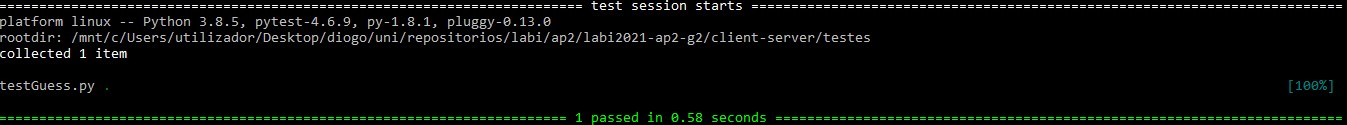
\includegraphics[width = 15 cm ]{testGuess_result.jpg}
\caption{Resultado do teste unitario}
\end{changemargin}
\end{figure}

\vspace{10mm}


A proxima função a testar é a  \textbf{stop\_client}, esta é chamada quando o cliente acerta e, assim, acaba o jogo. Esta função recebe o socket do cliente e a mensagem enviada pelo mesmo como argumentos. Inicialmente a partir da função, anteriormente testada, \textbf{find\_client\_id} acede ao id do cliente e em seguida depois de verificar possiveis erros como:
\begin{enumerate}
  \item Inconsistência do numero de jogadas.
  \item O valor de jogadas maximas exedido.
  \item Cliente não encontrado.
\end{enumerate}
devolve um dicionario de sucesso onde está presento o numero secreto.  

\begin{figure}[H]\label{fig:fig33}
\begin{changemargin}{-3.5cm}{-3.5cm}
\begin{tcolorbox}
\begin{lstlisting}[language=Python, inputencoding=utf8, breaklines=true, basicstyle=\small, showstringspaces=false]

import pytest

from server import (stop_client, gamers, guess_client)
from client import stop_action

def test():
	assert stop_client("abc", {"op": "STOP", "number": 60, "attempts": 20}) == { "op": "STOP", "status":True, "guess": 60} 
	assert stop_action("abc", 20) == ("--- Parabéns!!! Terminou o jogo em 20 tentativas ---")
	assert stop_client("abcdef", {"op": "STOP", "number": 32, "attempts": 20}) == { "op": "STOP", "status":False, "error": "Cliente inexistente" }
	assert stop_client("abc", {"op": "STOP", "number": 60, "attempts": 8}) == { "op": "STOP", "status":False, "error": "Numero de jogadas inconsistente" }
	increment = guess_client("abc", {"op": "GUESS", "number": 50}) #para incrementar a contagem, para ser possivel realizar a proxima testagem
	assert stop_client("abc", {"op": "STOP", "number": 60, "attempts": 21}) == { "op": "STOP", "status":False, "error": "Excedeu o numero maximo de tentativas" }
	
\end{lstlisting}
\end{tcolorbox}
\caption{Codigo do programa de teste}
\end{changemargin}
\end{figure}

Depois da função \textbf{stop\_client} ser executada a mensagem do resultado final é imprimida, esta provém da função \textbf{stop\_action} que é chamada na função \textbf{run\_client} do lado do cliente, quando o cliente acerta no número secreto e não ocorre qualquer erro nesse processo. A função \textbf{stop\_action} imprime uma mensagem onde aparece o número de jogadas efetuadas e se o cliente venceu ou perdeu, por fim, fecha o socket do cliente e termina o programa do mesmo. No teste acima apresentado aproveitou-se também para verificar esta função, para isso dentro da função trocou-se as instruções de \textbf{print} para \textbf{return}, assim abrindo a porta á simulação decorrendo a um \textbf{assert}. Como antes referido, na função \textbf{stop\_action} o programa é terminado e o socket do cliente fechado(que não foi aberto no teste), assim sendo impossível fazer qualquer teste unitário sem eliminar essas instruções, logo foram retiradas momentaneamente para os testes serem realizados. A instrução de limpeza do dicionário \textbf{gamers} também foi retirada, por razões similares às anteriores. As instruções eliminadas, mais à frente, na \autoref{sec.simulação} serão dadas a observar a funcionar.

Se observar o código de teste vê que se fez um GUESS de forma a aumentar em uma unidade o número na chave \textbf{attempts} guardado dentro do dicionário, assim o seu valor passa de 20 para 21, logo excede o \textbf{max\_attempts}, possibilitando o teste do erro 3 presenta na lista anterior. Por fim, foi considerado o dicionário \textbf{gamers}: \{"Manel": {"socket": "abc", "guess": 60, "max\_attempts": 20, "attempts": 20, "cipher": None\}\}.



\begin{figure}[H]\label{fig:fig34}
\begin{changemargin}{-3.5cm}{-3.5cm}
\center
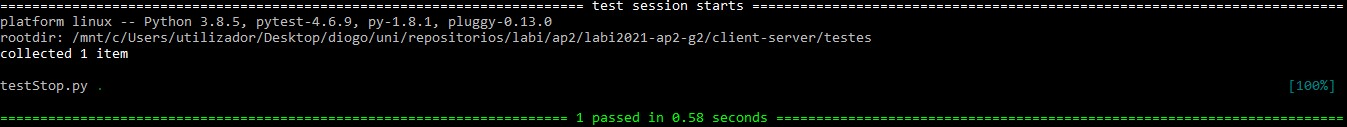
\includegraphics[width = 15 cm ]{testStop_result.jpg}
\caption{Resultado do teste unitario}
\end{changemargin}
\end{figure}

Comprova-se o funcionamento correto da função \textbf{stop\_client} e, parcialmente, da \textbf{stop\_action}.

\vspace{20mm}

As próximas funções a ser chamadas são as funções \textbf{new\_client}, \textbf{quit\_client} e \textbf{clean\_client}. Começando pela função \textbf{new\_client} esta é chamada logo no início do programa, quando o cliente decide iniciar jogo com ou sem encriptação entroduzindo no terminal "y" ou "n", introdozindo uma destas duas opções o client envia um socket e uma mensagem em formato j\_son com o seguinte texto $ \{"op": "START", "client\_id": sys.argv \footnote{sys.argv é utilizado para aceder à lista de argumentos passados pela linha de comandos em que o número é o local onde se posiciona o argumento que queremos aceder} \left [ 1 \right ], "cipher": cipherkey\_tosend \}$.
O servidor recebe a mensagem do cliente e chama a função \textbf{new\_client}, esta função é chamada sempre que o cliente envia "START" no campo "op", os argumentos da função são o socket e a resposta do cliente. O que a função faz é :
\begin{enumerate}
\item Verificar se o cliente já existe.
\item Guardar os valores essenciais do jogo no dicionário gamers.
\item Enviar uma mensagem ao cliente com o número de jogadas máximas
\end{enumerate}
Caso o cliente já exista a função deve devolver uma mensagem de erro, caso não exista deve devolver uma mensagem ao cliente com o número máximo de jogadas . Neste teste também usamos o cliente Manel.



\begin{figure}[H]
\begin{changemargin}{-3.5cm}{-3.5cm}
\begin{tcolorbox}
\begin{lstlisting}[language=Python, inputencoding=utf8, breaklines=true, basicstyle=\small, showstringspaces=false]

import pytest

from server import (update_file, find_client_id, new_client, quit_client, gamers, clean_client)

def test():
	assert new_client("abc", {"op": "START", "client_id": "Manel", "cipher": None}) == { "op": "START", "status":False, "error": "cliente existente" }
	assert new_client("abcd", {"op": "START", "client_id": "Paula", "cipher": None}) == { "op": "START", "status":True, "max_attempts": gamers["Paula"]["max_attempts"] }
	assert quit_client("abcd", {"op": "QUIT"}) == { "op": "QUIT", "status":True}
	assert quit_client("abcde", {"op": "QUIT"}) == { "op": "QUIT", "status":False, "error": "cliente inxistente" }
	assert clean_client("abc") == True
	assert clean_client("4515") == False
	
\end{lstlisting}
\end{tcolorbox}
\caption{codigo do programa de teste}\label{fig:fig35}
\end{changemargin}
\end{figure}

Depois da função \textbf{new\_client} testamos a função \textbf{quit\_client}, esta função é chamada sempre que o cliente enviar a seguinte mensagem $ \{"op": "QUIT"\}$. A função recebe dois argumentos: o client\_sock e a mensagem do cliente. Se o client já está registado no dicionário gamers, a função tem três operações a fazer:
\begin{enumerate}
\item Atualizar o ficheiro \textbf{report.csv} através da função update\_file.
\item Eleminar o cliente do dicionário gamers, através da função clean\_client.
\item Enviar uma mensagem ao cliente com a operação Quit e status \textbf{True}
\end{enumerate}
Caso o cliente não esteja registado no dicionário só deve enviar uma mensagem de erro ao cliente a informar que o cliente é inexistente.

Por fim na figura ~\ref{fig:fig35} é testada também a função clean\_client que já foi referido anteriormente qual é o seu objetivo, mas na mesma podemos ver os valores que devolve e perceber o seu significado. Como "abc" neste teste é o socket do cliente Manel a função devolve "True" quando este é passado como argumento, quando damos como argumento à função um socket que ainda não foi guardado ela devolve False.


\begin{figure}[H]
\begin{changemargin}{-3.5cm}{-3.5cm}
\center
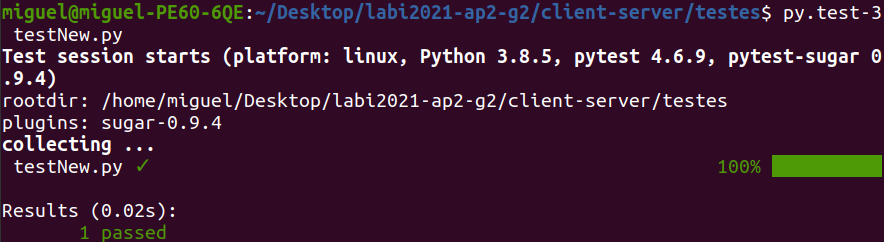
\includegraphics[width = 15 cm ]{testNew_result.png}
\caption{Resultado do teste unitario}\label{fig:36}
\end{changemargin}
\end{figure}

Vai ser testada a função validate\_response do cliente, esta função consiste em validar a resposta recebida do servidor e caso na mensagem recebida o campo status for True a função devolve True, se a mensagem recebida conter no campo status o valor booleano False, a função deve retornar uma mensagem de erro com o erro que recebe do servidor, na figura \ref{fig:37} podemos ver o código do teste que tem todos os casos passíveis de erro.

\begin{figure}[H]
\begin{changemargin}{-3.5cm}{-3.5cm}
\begin{tcolorbox}
\begin{lstlisting}[language=Python, inputencoding=utf8, breaklines=true, basicstyle=\small, showstringspaces=false]

import pytest

from client import validate_response

def test():
	assert validate_response("abc", { "op": "STOP", "status":False, "error": "Cliente inexistente" }) == "--- Erro: " + "Cliente inexistente" + " ---"
	assert validate_response("abcs", { "op": "STOP", "status":False, "error": "Excedeu o numero maximo de tentativas" })  == "--- Erro: " + "Excedeu o numero maximo de tentativas" + " ---"
	assert validate_response("avdsefg", { "op": "STOP", "status":False, "error": "Numero de jogadas inconsistente" }) == "--- Erro: " + "Numero de jogadas inconsistente" + " ---"
	assert validate_response("ghjkl", {"op":"Sair", "status": False, "error": "Operação inexistente (operações possivesis: \"START\", \"GUESS\", \"QUIT\", \"STOP\")"}) == "--- Erro: " + "Operação inexistente (operações possivesis: \"START\", \"GUESS\", \"QUIT\", \"STOP\")" + " ---"
	assert validate_response("1234",  {"op": "GUESS", "status":False, "error": "Tem de inserir um valor do tipo inteiro positivo" })	== "--- Erro: " + "Tem de inserir um valor do tipo inteiro positivo" + " ---"
	assert validate_response("aghsj", { "op": "GUESS", "status":False, "error": "Valor fora dos limites (0 <= number <= 100)" }) == "--- Erro: " + "Valor fora dos limites (0 <= number <= 100)" + " ---"
	assert validate_response("dscfew", { "op": "START", "status":True, "max_attempts": 22 }) == True
	assert validate_response("sgdhensm", { "op": "QUIT", "status":True}) == True
	assert validate_response("fdfwd", { "op": "GUESS", "status":True, "result": 20 }) == True
	
\end{lstlisting}
\end{tcolorbox}
\caption{codigo do programa de teste}\label{fig:37}
\end{changemargin}
\end{figure}


\begin{figure}[H]
\begin{changemargin}{-3.5cm}{-3.5cm}
\center
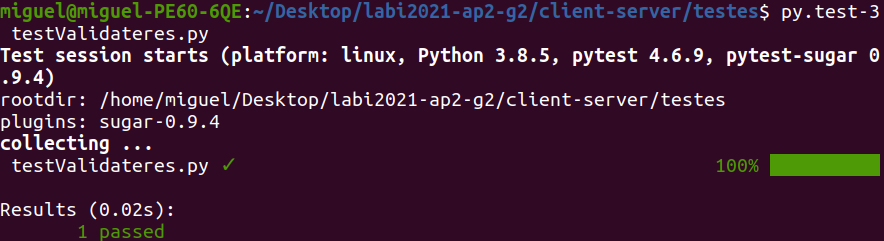
\includegraphics[width = 15 cm ]{testValidateres_result.png}
\caption{Resultado do teste unitario}\label{fig:38}
\end{changemargin}
\end{figure}

No cliente a função quit\_action tem 2 argumentos, o primeiro o client\_sock e o segundo a resposta do servidor, o segundo argumento não tem influência o primeiro tem para uma das operações. A função têm 3 operações a fazer, que são:
\begin{enumerate}
  \item Fechar o socket
  \item Dar return à mensagem "Desistiu com sucesso"
  \item Terminar o programa do client
\end{enumerate}


\begin{figure}[H]
\begin{changemargin}{-3.5cm}{-3.5cm}
\begin{tcolorbox}
\begin{lstlisting}[language=Python, inputencoding=utf8, breaklines=true, basicstyle=\small, showstringspaces=false]

import pytest

from client import quit_action


def test():
	assert quit_action("abcd", 3) == "--- Desistiu com sucesso ---"
	assert quit_action("dfghb", 7) == "--- Desistiu com sucesso ---"
\end{lstlisting}
\end{tcolorbox}
\caption{codigo do programa de teste}\label{fig:39}
\end{changemargin}
\end{figure}

Na figura \ref{fig:39} está o código que faz a verificação do return da função qui\_action.


\begin{figure}[H]
\begin{changemargin}{-3.5cm}{-3.5cm}
\center
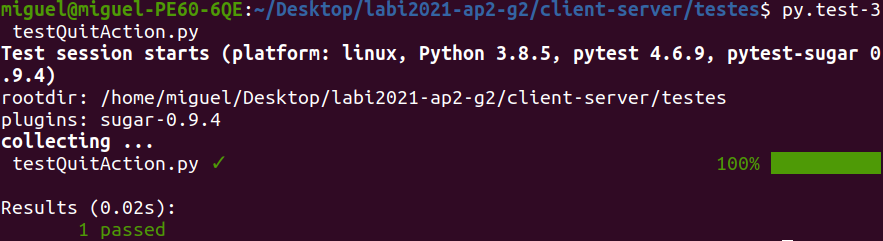
\includegraphics[width = 15 cm ]{testQuitAction_result.png}
\caption{Resultado do teste unitario}
\end{changemargin}
\end{figure}

\begin{section}{Simulação de uma interação cliente-servidor}
\label{sec.simulação}

Em vista simular uma possível interação entre cliente e servidor, usou-se a funcionalidade \textbf{\ac{ipdb}}, assim podendo ter mais acesso em tempo real às variáveis do programa. A partir do par de imagens a baixo colocadas, pode-se verificar:
\begin{enumerate}
\item É inicialmente perguntado se o cliente quer usar encriptação, essa resposta pode ser dada tanto em maiúscula como em minuscula, seguida ou precedida por espaços, como qualquer resposta durante a interação.
\item Depois de enviado o pedido de \textbf{START}, que irá registar cliente na lista de clientes do servidor, uma resposta é recebida onde se verifica o sucesso da operação.
\item O jogo começa e o número máximo de jogadas é apresentado ao cliente.
\item O cliente depois de introduzir um número, esse é armazenado na variável \textbf{number}. Depois do pedido de \textbf{GUESS} pela parte do programa do cliente, o servidor responde com um dicionário de sucesso e o resultado da comparação entre o número dado pelo cliente e o número secreto, esse mesmo é imprimido no ecrã do jogador.
\item O número de tentativas efetuadas é atualizado, neste caso fez-se o print do registo do lado do cliente que é crucial estar correto, pois tem de ser igual à contagem feita pelo servidor.
\item Finalmente, quando se acerta no número secreto, neste caso o 24, a operação \textbf{STOP} é requerida ao servidor, que envia, neste caso, uma resposta afirmativa, assim, desencadeado a apresentação do resultado do jogo, o fecho do socket cliente e terminação do programa.

\end{enumerate}

\begin{figure}[H]
\begin{changemargin}{-3.5cm}{-3.5cm}
\center
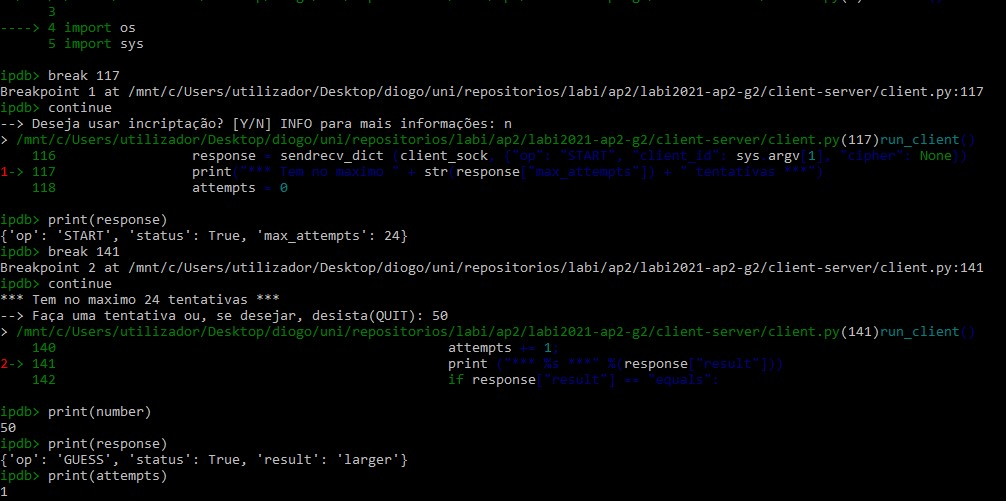
\includegraphics[width = 15 cm ]{p1sim.jpg}
\end{changemargin}
\end{figure}

\begin{figure}[H]
\begin{changemargin}{-3.5cm}{-3.5cm}
\center
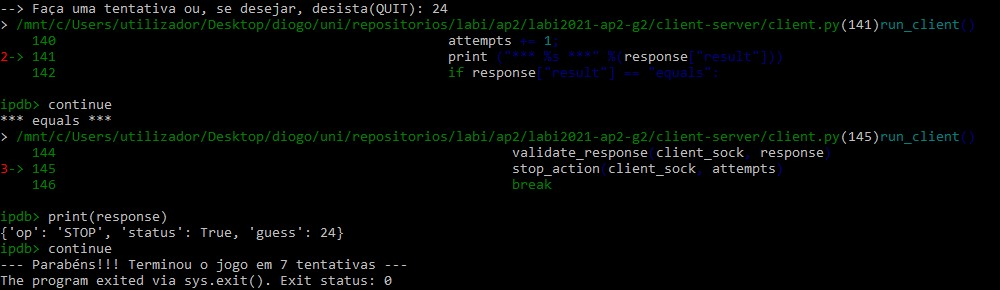
\includegraphics[width = 15 cm ]{p2sim.jpg}
\caption{Resultado da simulação}
\end{changemargin}
\end{figure}

Esta simulação possibilita, tanto a visualização de um possível uso dos programas criados, como o funcionamento dos mesmos.

Aproveito para mostrar uma função adicional criada chamada \textbf{INFO}. Quando o cliente quiser mais informação sobre o funcionamento do jogo, basta digitar INFO (ou info) e será-lhe apresentado um pequeno texto(ver figura \ref{fig:info} ) que poderá esclarecer qualquer dúvida existente.

\begin{figure}[H]
\begin{changemargin}{-3.5cm}{-3.5cm}
\center
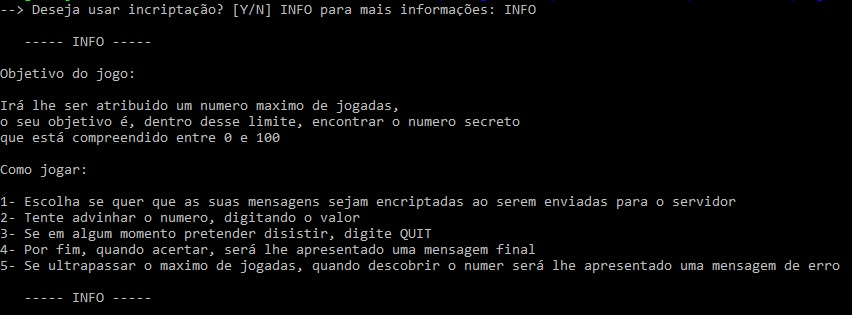
\includegraphics[width = 15 cm ]{info.jpg}
\caption{Resultado da operação \textbf{INFO}}
\label{fig:info}
\end{changemargin}
\end{figure}


\end{section}
\section{Segurança - uso de incriptação}
\label{sec.segurança}

De forma a tornar a comunicação entre o clientre e o servidor mais segura, quando o programa cliente é iniciado é perguntado se quer usar incriptação, ou não. Em caso que o cliente o deseje, todos os numeros trocados entre o programa cliente e servidor são todos protegidos a partir de incriptação. basicamente antes de se enviar o dicionario para o respetivo destinatario, usa-se a função \textbf{encrypt\_intvalue} para incriptar os valores pretendidos, para isso é criada uma cifra de 16 bytes aleatoria, que entra como argumento na função, para alem do valor a incriptar. No lado do distinatario a função  \textbf{decrypt\_intvalue} desincripta o valor para, assim, poder ser usado da forma tipica.

Para testar este sistema de incriptação / desincriptação usou-se a funcionalidade  \textbf{\ac{ipdb}} que nos permitiu visualizar o valor de variaveis durante o funcionamento do programa. Estes testes foram feitos no programa cliente, sendo possivel verificar a correção do servidor a partir das resposta recebidas.

\begin{figure}[H]
\begin{changemargin}{-3.5cm}{-3.5cm}
\center
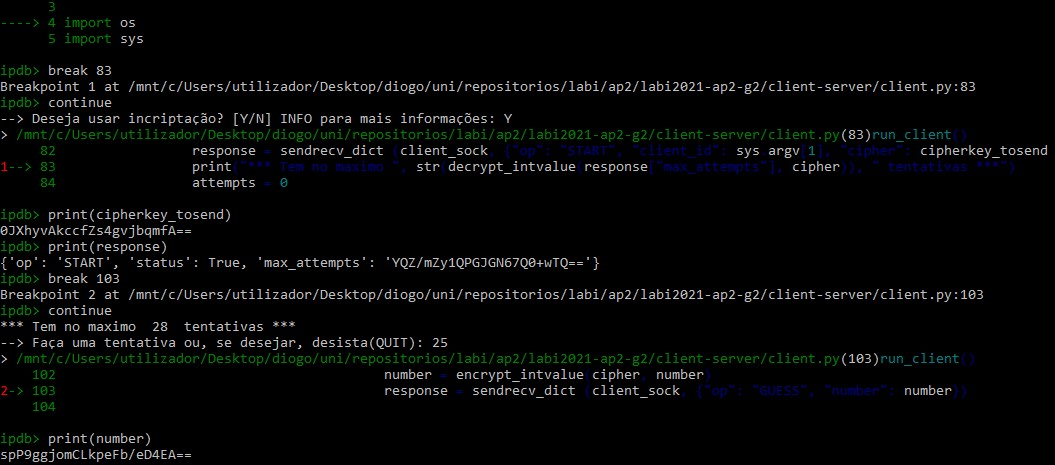
\includegraphics[width = 15 cm ]{incriptacao.jpg}
\caption{Resultado do teste ipdb da segurança}
\end{changemargin}
\end{figure}

Como é possível visualizar na imagem acima, uma cifra é criada, ver resultado de \textbf{print(cipherkey\_tosend)}, e a respostas do servidor também veem encriptadas, ver \textbf{print(response)} onde aparece o número máximo de tentativas encriptado, logo a seguir a mesma é desencriptada, ver a mensagem onde aparece o 28 como número máximo de tentativas. Para reforçar a ideia, ainda se fez o \textbf{print(number)} que seria, em decimal, 25, mas aparece , depois de encriptado, como ``spP9ggjomCLkpeFb/eD4EA==''.

Depois deste pequeno teste, conclui-se que o sistema de encriptação / desencriptação está a funcionar como esperado.



\chapter{Análise geral}
\label{chap.analise geral}

Resumindo, o que foi possível concluir depois dos testes e simulações realizadas? Primeiramente, asseguramos que a iniciação dos programas criados são o mais robustos possível, tratando os erros gerados de forma a se tornarem em mensagens que possam elucidar o cliente. Depois de todos os programas a correr, era crucial que as funções implementadas servissem para o que forma desenhadas, na \autoref{sec.funções} asseguramos que as funções essenciais funcionam como esperado, tanto a nível de retornos como de deteção de erros. De seguida na autoref{sec.simulação} mostramos aquilo que poderia ser uma interação cliente / servidor, usando a ferramenta ipdb do python fomos um pouco mais além e mostramos que realmente as variáveis e dicionários, que vão flutuando durante o percorrer dos programas, eram atualizadas. Por fim, testou-se a parte da segurança, o sistema de encriptação e de desencriptação tinham de estar a funcionar de forma perfeita, assim fazendo com que a comunicação não fosse perdida ou modificada em qualquer momento, assim, viu-se que tal está assegurado. 


\chapter{Conclusões}
\label{chap.conclusao}
Agora, estamos na posição de afirmar que os programas funcionam como esperado, a robustez têm bastante abrangência e uma comunicação mais segura entre cliente / servidor também é possível. Os objetivos delineados para este projeto foram alcançados com sucesso.

\chapter*{Contribuições dos autores}
As funções essenciais foram maioritariamente feitas por DM, a implementação da segurança e das funções de escrita do report csv foram realizadas por MA. O relatório foi escrito sem grande distensão.

Contribuições: DM- 50\%, MG- 50\%.

%%%%%%%%%%%%%%%%%%%%%%%%%%%%%%%%%
\chapter*{Acrónimos}
\begin{acronym}
\acro{ua}[UA]{Universidade de Aveiro}
\acro{miect}[MIECT]{Mestrado Integrado em Engenharia de Computadores e Telemática}
\acro{lei}[LEI]{Licenciatura em Engenharia Informática}
\acro{ipdb}[ipdb]{IPython-enabled Python Debugger}
\acro{labi}[LABI]{Laboratórios de Informática}
\acro{uc}[UC]{unidade curricular}
\acro{csv}[CSV]{Comma-separated values}
\end{acronym}

\medskip
%%%%%%%%%%%%%%%%%%%%%%%%%%%%%%%%%
\printbibliography

\end{document}
